% !TEX encoding = UTF-8 Unicode
%%%% SLIDES FOR PRESENTATION %%%
\documentclass[notes=hide]{beamer}

%%%% ALL SLIDES (WHEN PREPARING SLIDES) %%%
%\documentclass[handout]{beamer}

\usepackage[all]{xy}
\usepackage{hyperref}
\usepackage{setspace}
\setbeamertemplate{navigation symbols}{}

% adding tikz to draw arrows, etc
\usepackage{tikz}  
\usetikzlibrary{arrows,shapes,backgrounds}
\usepackage{soul} % package to strike out text



\begin{document}
	

  


\begin{frame}
	\frametitle{Text as data}
	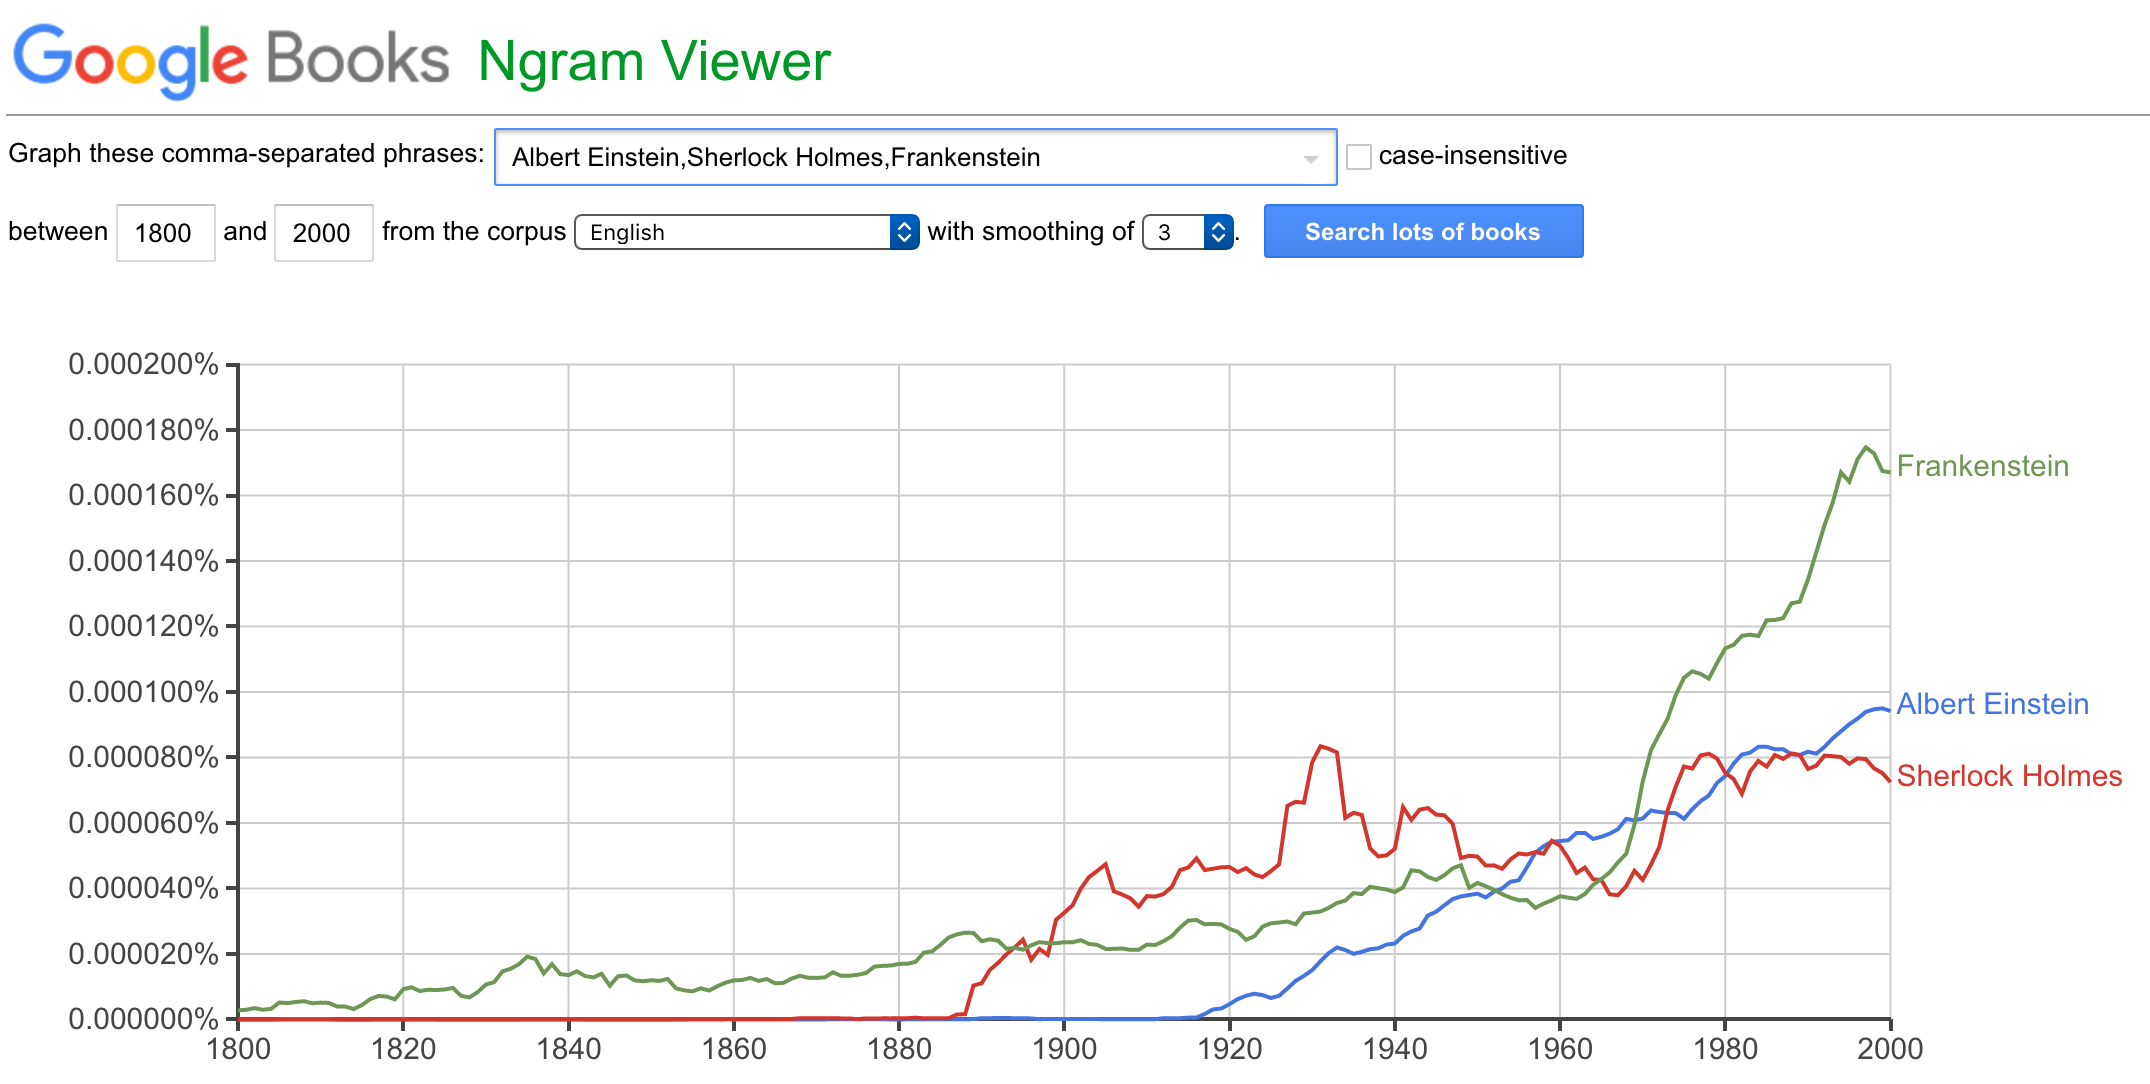
\includegraphics[width=1\linewidth]{figures/motivation3.png}
\end{frame}

\begin{frame}
	\frametitle{Text as data}
	
\includegraphics[width=1\linewidth]{figures/motivation4.jpg}
\end{frame}

\begin{frame}
	\frametitle{Basic QTA Process: Texts $\rightarrow$ Feature matrix $\rightarrow$ Analysis}
	%  \vspace{-.5in}
	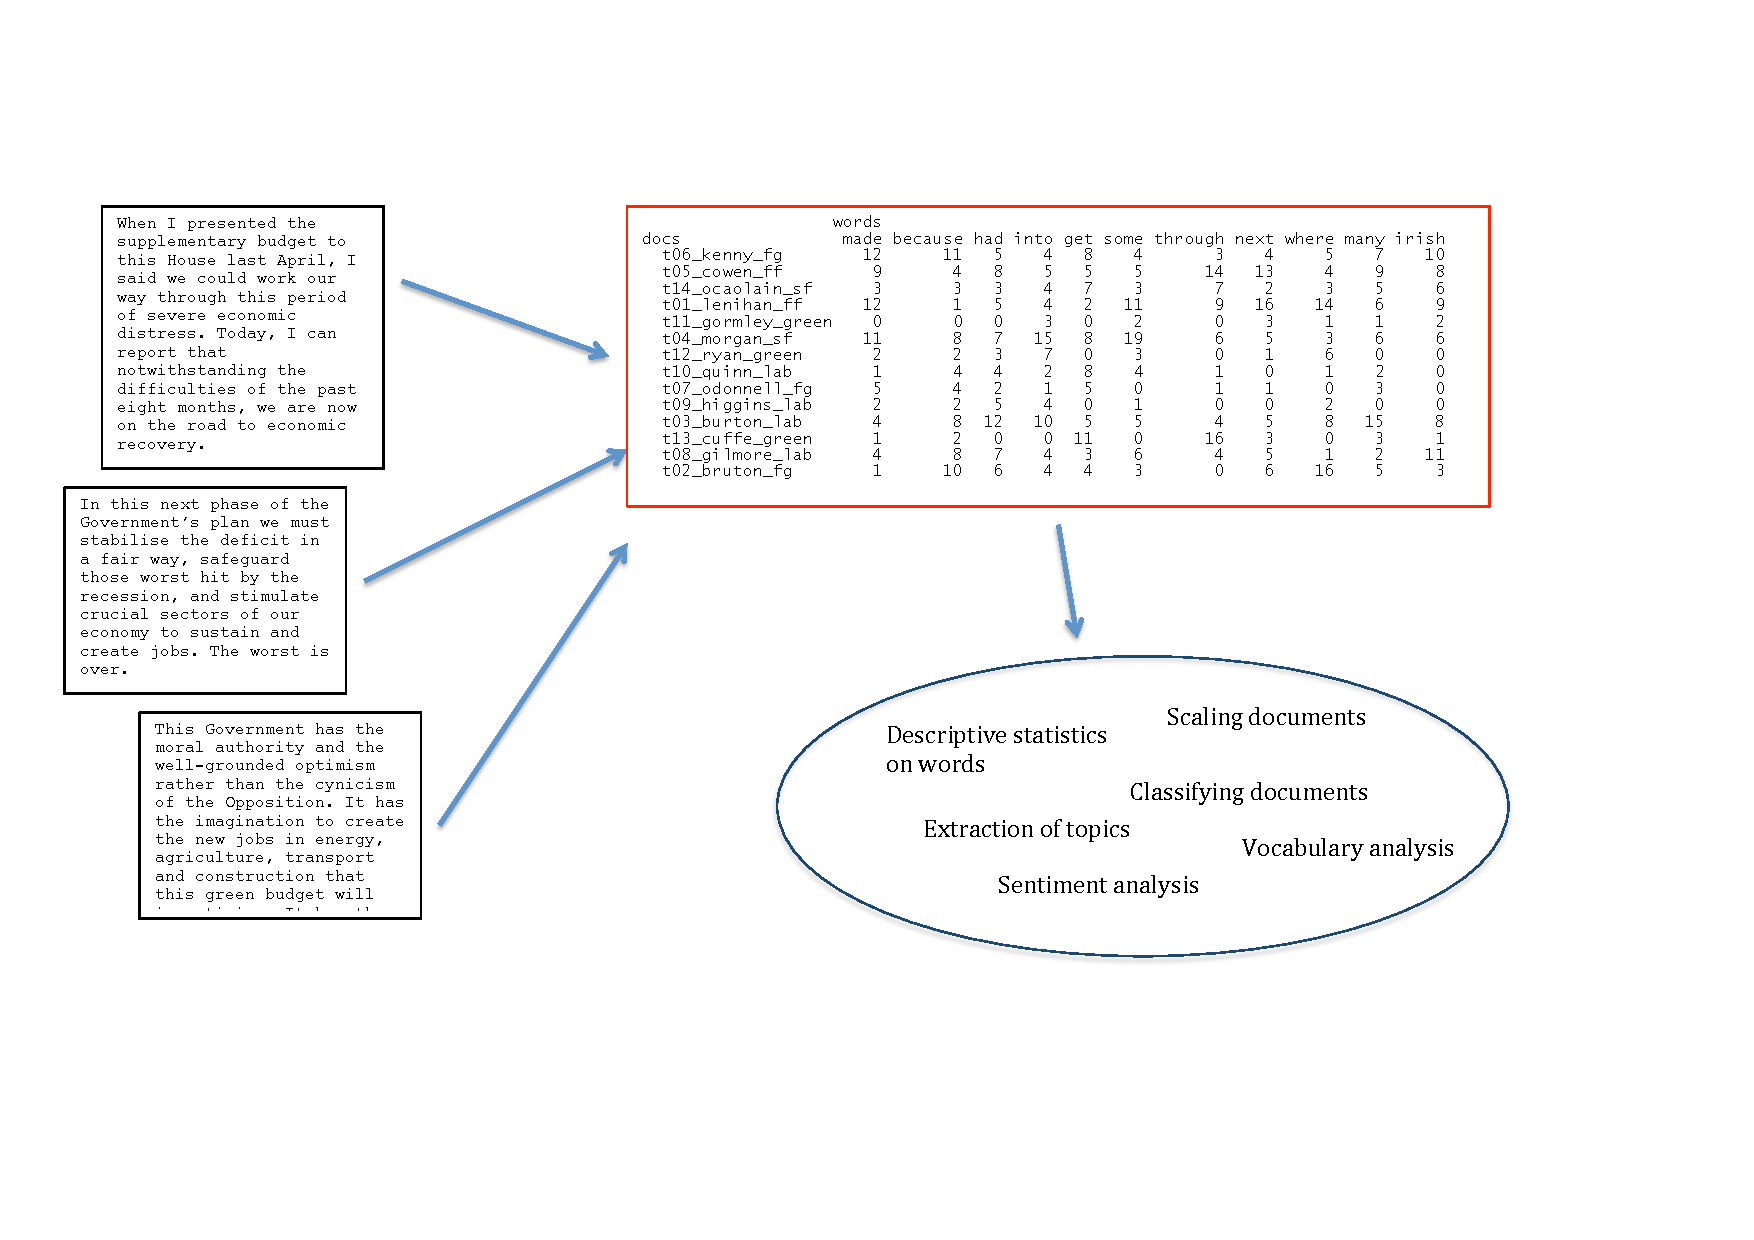
\includegraphics[width=11.5cm]{figures/workflow.pdf}
\end{frame}

\begin{frame}
	\frametitle{Outline}
	\begin{itemize}
		\item Foundations
		\item Examples
		\item Key terms in quantitative text analysis
		\item Justifying a term/feature frequency approach
		\item Selecting texts / defining documents
		\item Selecting features
	\end{itemize}
\end{frame}



\begin{frame}
	\frametitle{Why quantitative text analysis?}
	
	Justin Grimmer's haystack metaphor: \alert{QTA improves reading}
	
	\begin{itemize}[<+->]
		\item Analyzing a straw of hay: understanding the meaning of a sentence
		\begin{itemize}
			\item Humans are great! But computer struggle
		\end{itemize}
		\item Organizing the haystack: describing, classifying, scaling texts
		\begin{itemize}
			\item Humans struggle. But computers are great!
			\item (What this section is about)
		\end{itemize}
	\end{itemize}
	\uncover<+->{\alert{Principles of quantitative text analysis} (Grimmer \& Stewart, 2013)}
	\begin{enumerate}[<+->]
		\item All quantitative models are wrong -- but some are useful
		\item Quantitative methods for text amplify resources and augment humans
		\item There is no globally best method for automated text analysis
		\item Validate, validate, validate
	\end{enumerate}
	
\end{frame}

\begin{frame}
	\frametitle{Quantitative text analysis requires assumptions}
	\begin{enumerate}[<+->]
		\setlength{\itemsep}{1ex}
		\item Texts represent an observable implication of some
		underlying characteristic of interest
		\begin{itemize}
			\item An attribute of the author
			\item A sentiment or emotion
			\item Salience of a political issue
		\end{itemize}
		\item Texts can be represented through extracting their
		\emph{features}
		\begin{itemize}
			\item most common is the \alert{bag of words} assumption
			\item many other possible definitions of ``features'' (e.g. word embeddings)
		\end{itemize}
		\item A \alert{document-feature matrix} can be analyzed using
		quantitative methods to produce meaningful and valid estimates of
		the underlying characteristic of interest
	\end{enumerate}
\end{frame}

\begin{frame}
	%  \frametitle{Basic QTA Process: Texts $\rightarrow$ Feature matrix $\rightarrow$ Analysis}
	%  \vspace{-.5in}
	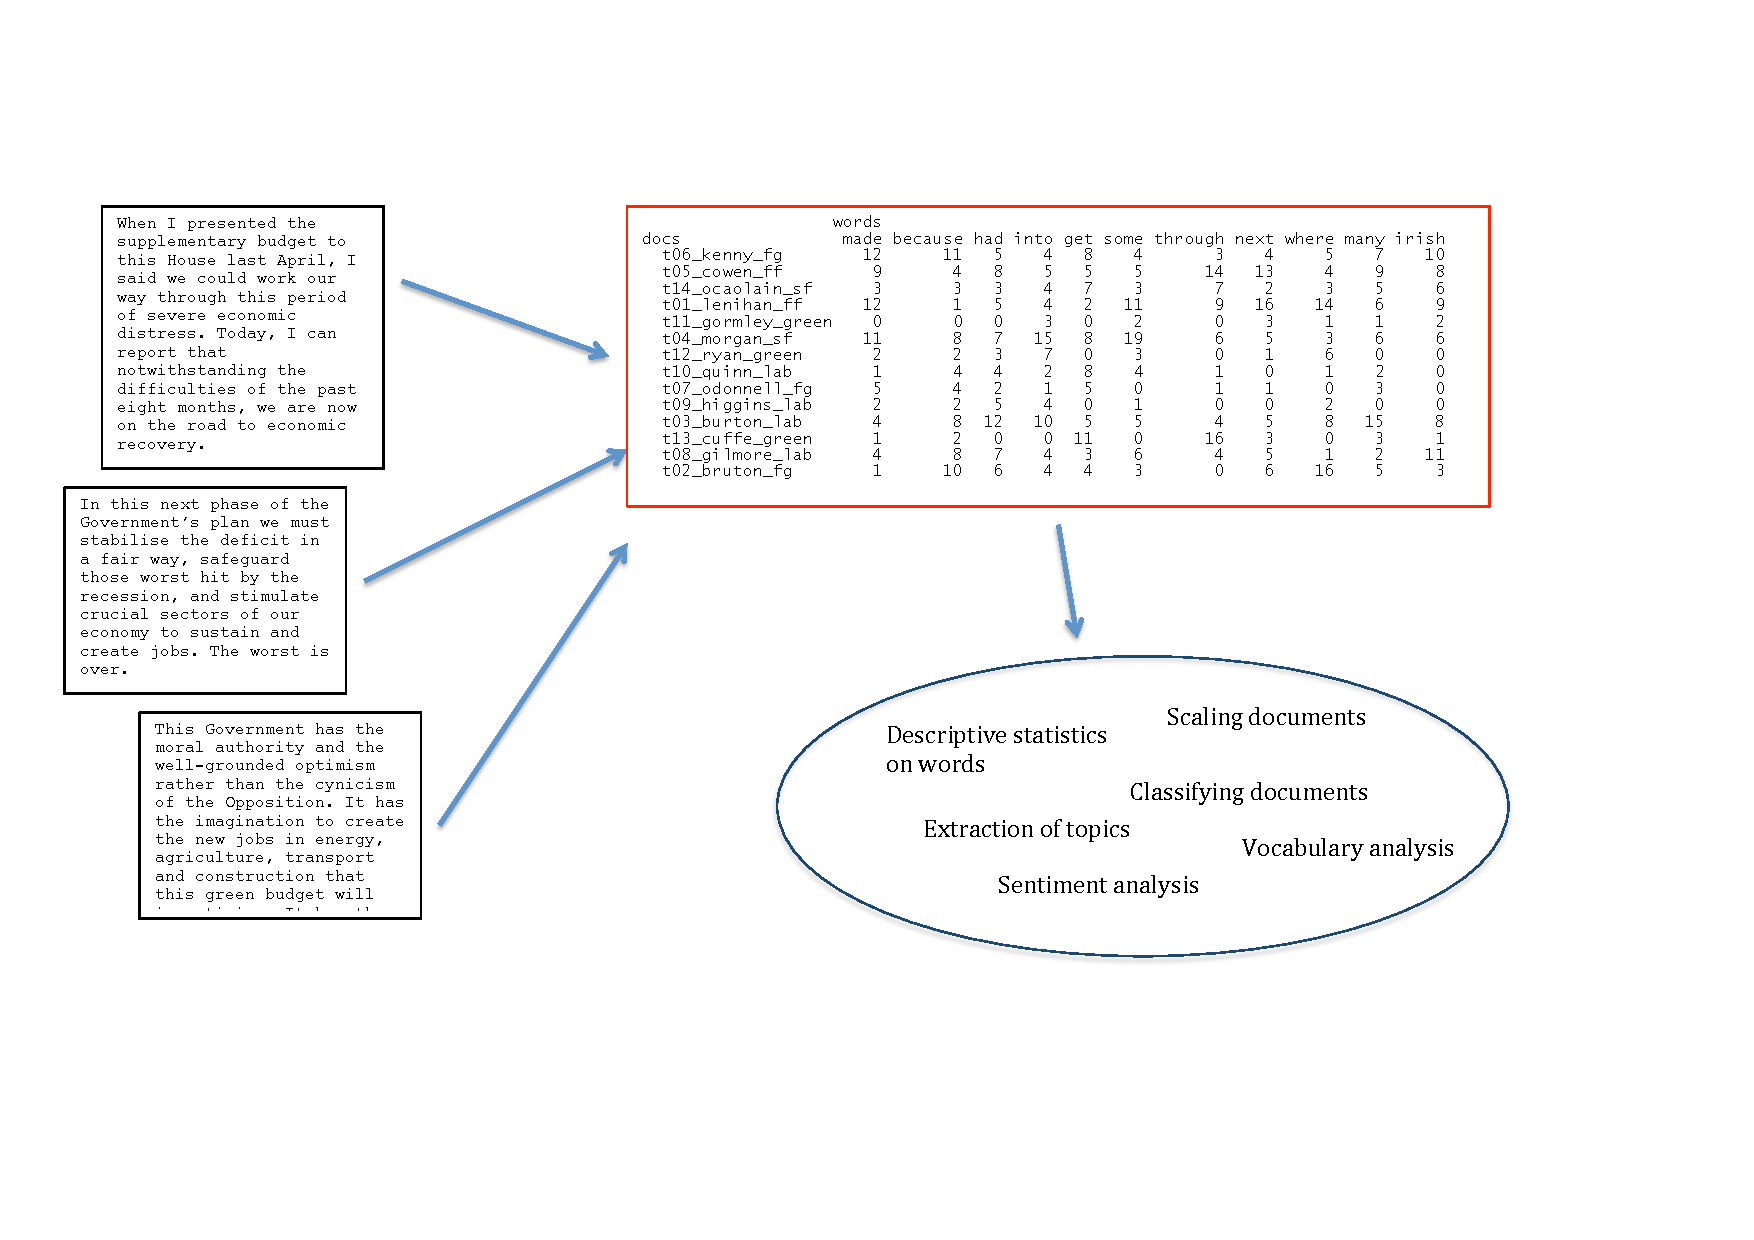
\includegraphics[width=11.5cm]{figures/workflow.pdf}
\end{frame}


\begin{frame}
	\frametitle{Key feature of quantitative text analysis}
	\begin{enumerate}[<+->]
		\setlength{\itemsep}{1.5ex}
		\item \alert{Selecting texts}: Defining the \emph{corpus}
		\item \alert{Conversion} of texts into a common electronic format
		\item \alert{Defining documents}: deciding what will be the
		documentary unit of analysis
	\end{enumerate}
\end{frame}

\begin{frame}
	\frametitle{Key feature of quantitative text analysis (cont.)}
	\begin{enumerate}[<+->]
		\setcounter{enumi}{3}
		\setlength{\itemsep}{1.5ex}
		\item \alert{Defining features}.  These can take a variety of forms,
		including tokens, equivalence classes of tokens (dictionaries),
		selected phrases, human-coded segments (of possibly variable
		length), linguistic features, and more.
		\item \alert{Conversion of textual features into a quantitative
			matrix}
		\item A \alert{quantitative or statistical procedure} to extract information
		from the quantitative matrix
		\item \alert{Summary} and interpretation of the quantitative results
	\end{enumerate}
\end{frame}


\begin{frame}
	\frametitle{Descriptive text analysis}
	
	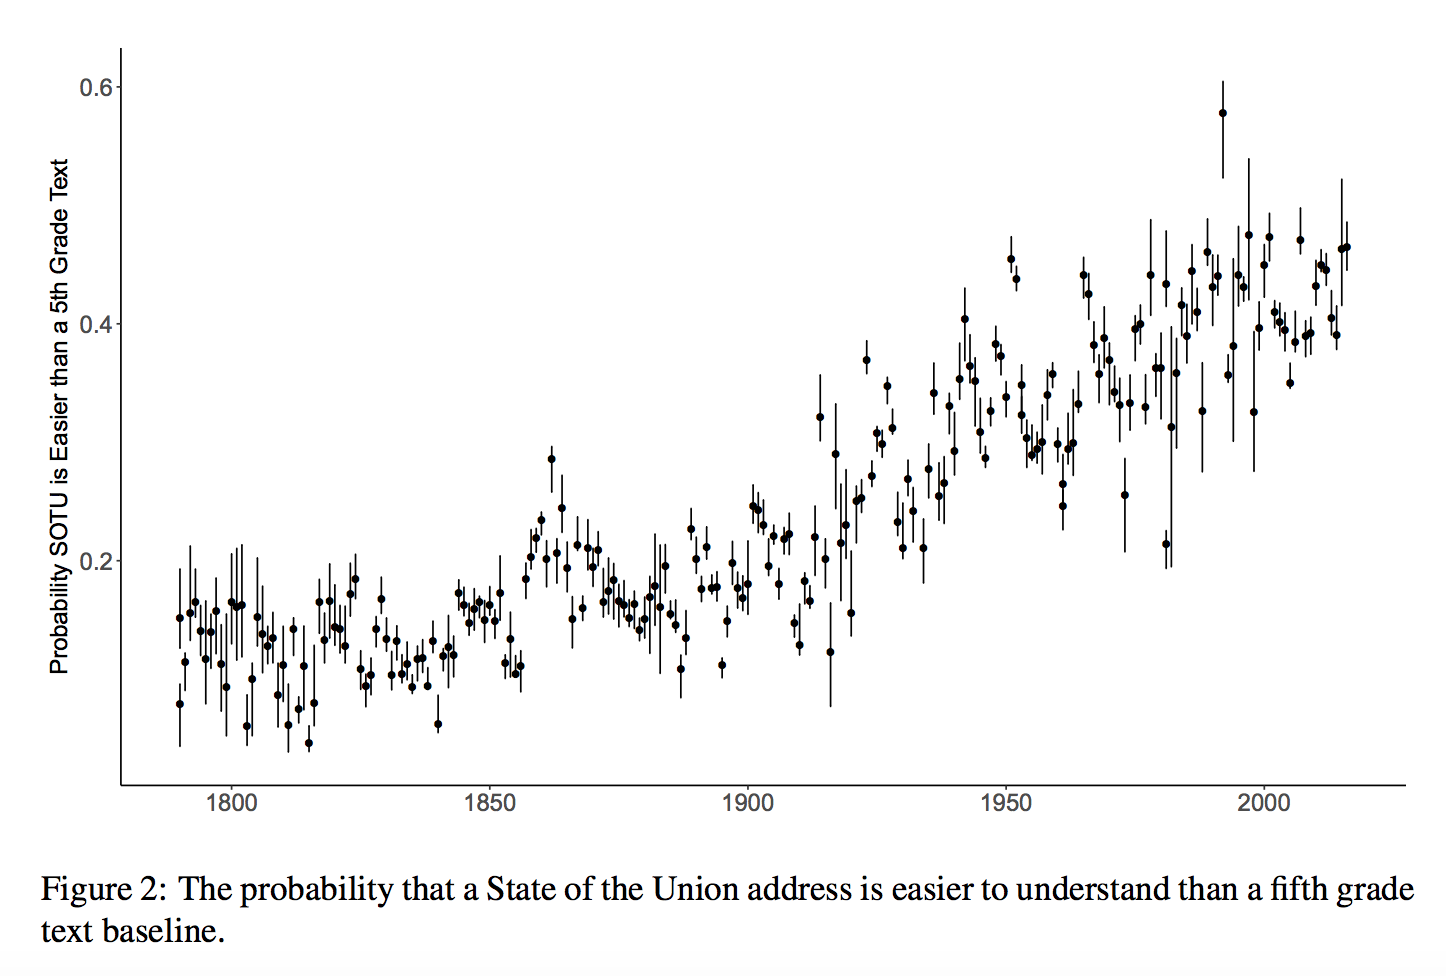
\includegraphics[width=1\textwidth]{figures/readability.png}\\
	\centering Benoit, Munger \& Spirling (2017)
	
	
\end{frame}


\begin{frame}
	\frametitle{Ideological scaling (Lauderdale \& Herzog, PA 2016)}
	\centering 
	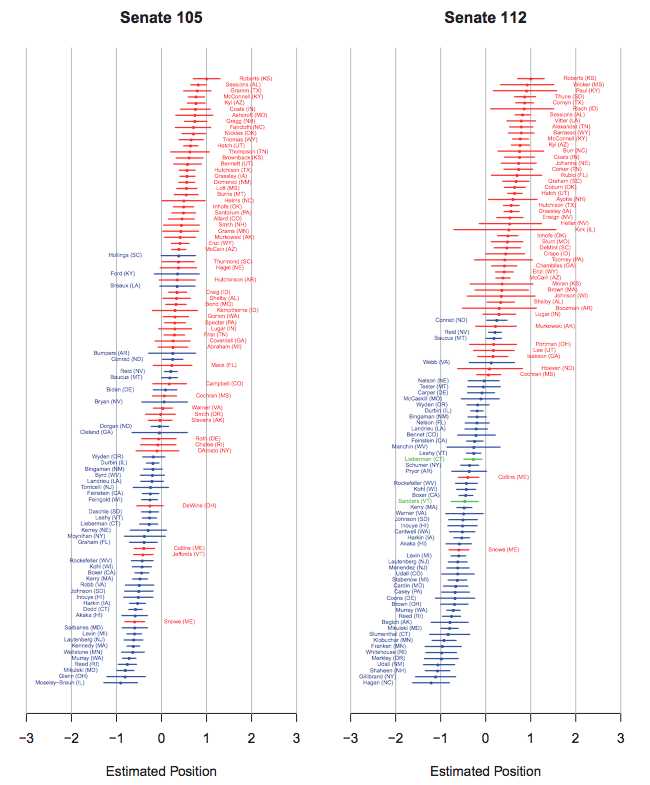
\includegraphics[height=.9\textheight]{figures/lauderdale-herzog-PA.png}
	
\end{frame}

\begin{frame}
	\frametitle{Document classification into unknown categories}
	Bauer, Barber\'{a} \textit{et al}, \textit{Political Behavior}, 2016.
	\begin{itemize}[<+->]
		\item Data: General Social Survey (2008) in Germany
		\item Responses to questions: \textit{Would you please tell me what you associate with the term ``left''? and would you please tell me what you associate with the term ``right''?}
		\item Open-ended questions minimize priming and potential interviewer effects
		\item Automated text analysis to discover unknown categories and classify responses
	\end{itemize}
\end{frame}

\begin{frame}
	\frametitle{Document classification into unknown categories}
	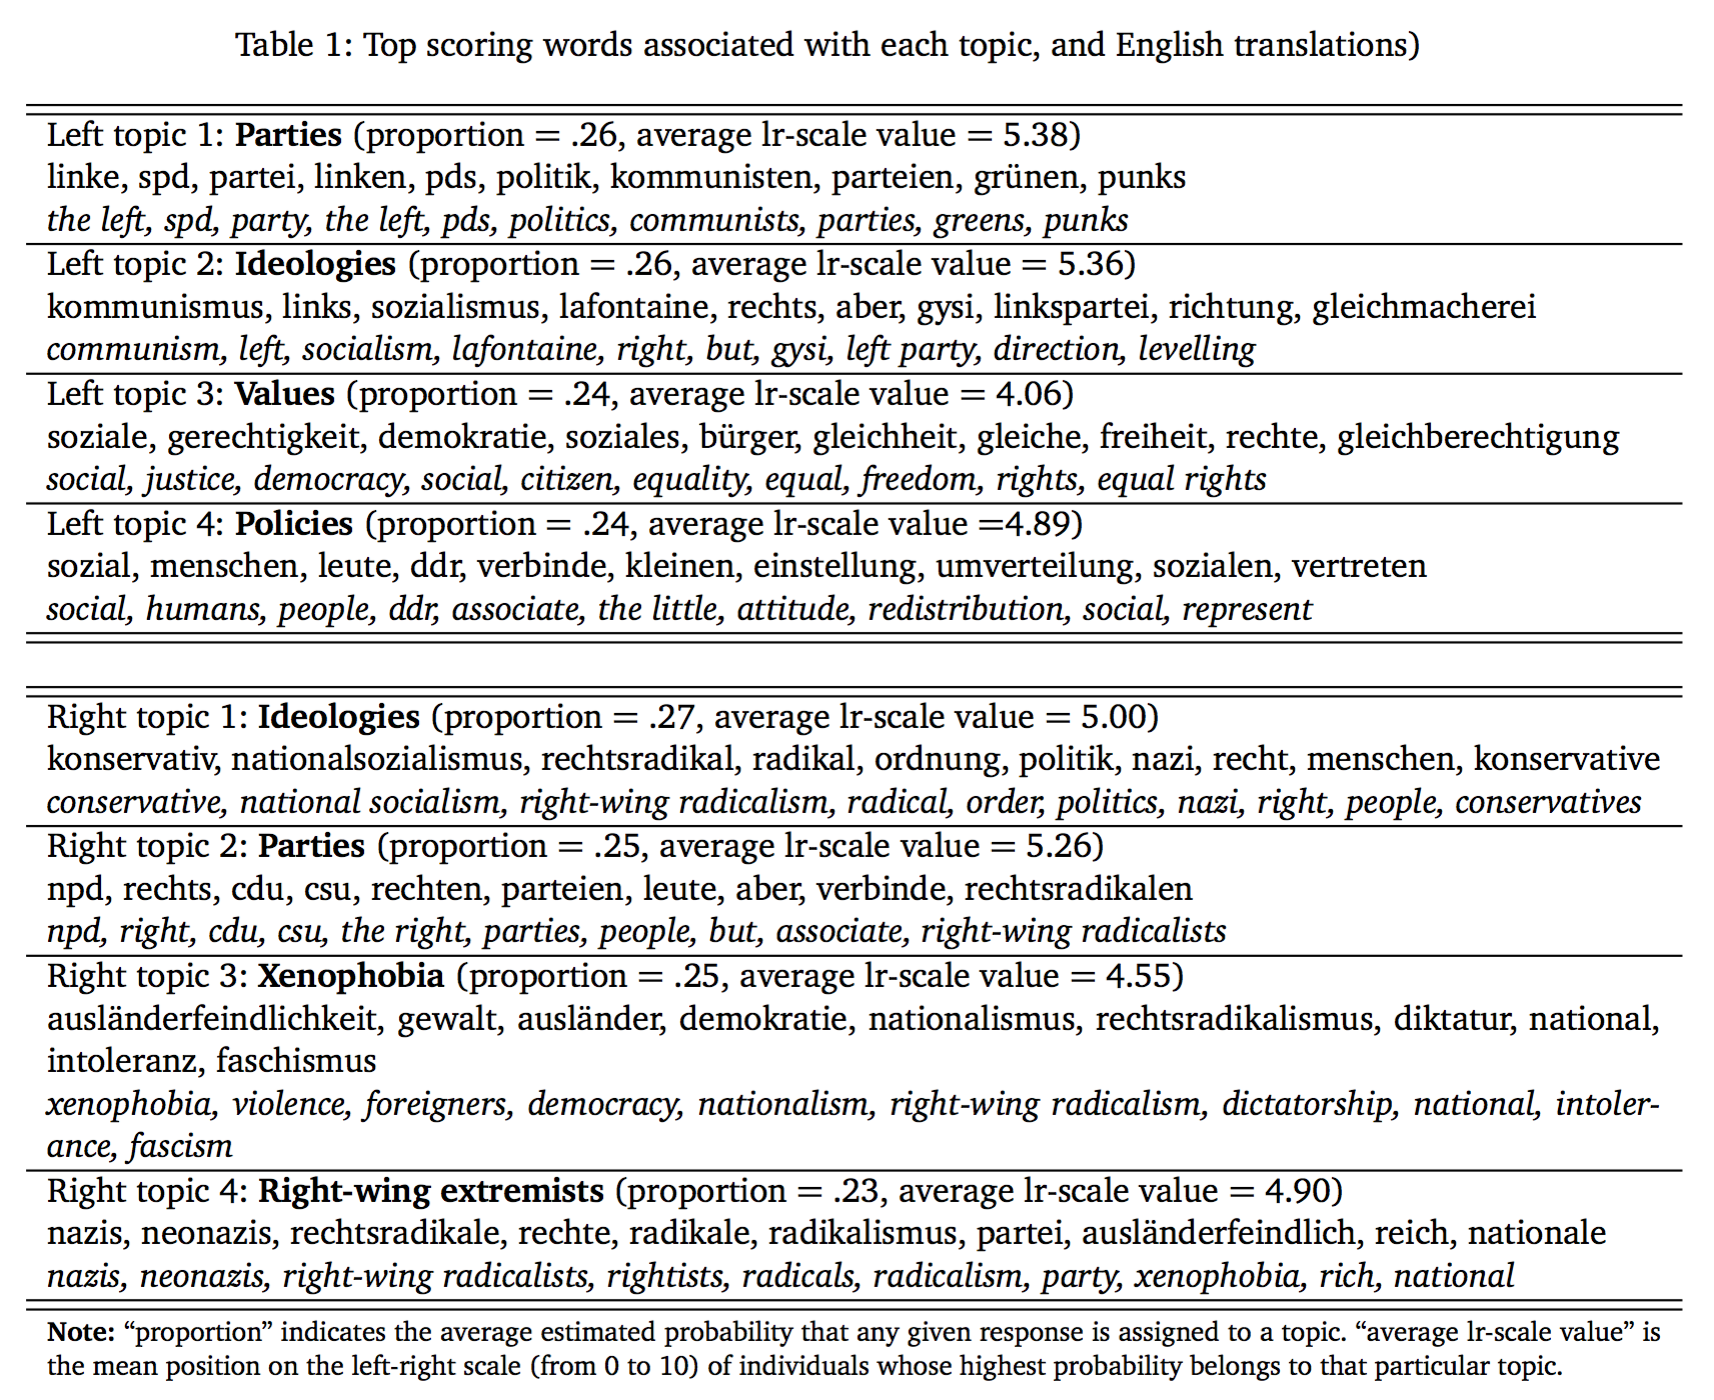
\includegraphics[width=.9\textwidth]{figures/pobe1.png}\\
	Bauer, Barber\'{a} \textit{et al}, \textit{Political Behavior}, 2016.
\end{frame}



\begin{frame}
	\frametitle{Basic QTA Process: Texts $\rightarrow$ Feature matrix $\rightarrow$ Analysis}
	%  \vspace{-.5in}
	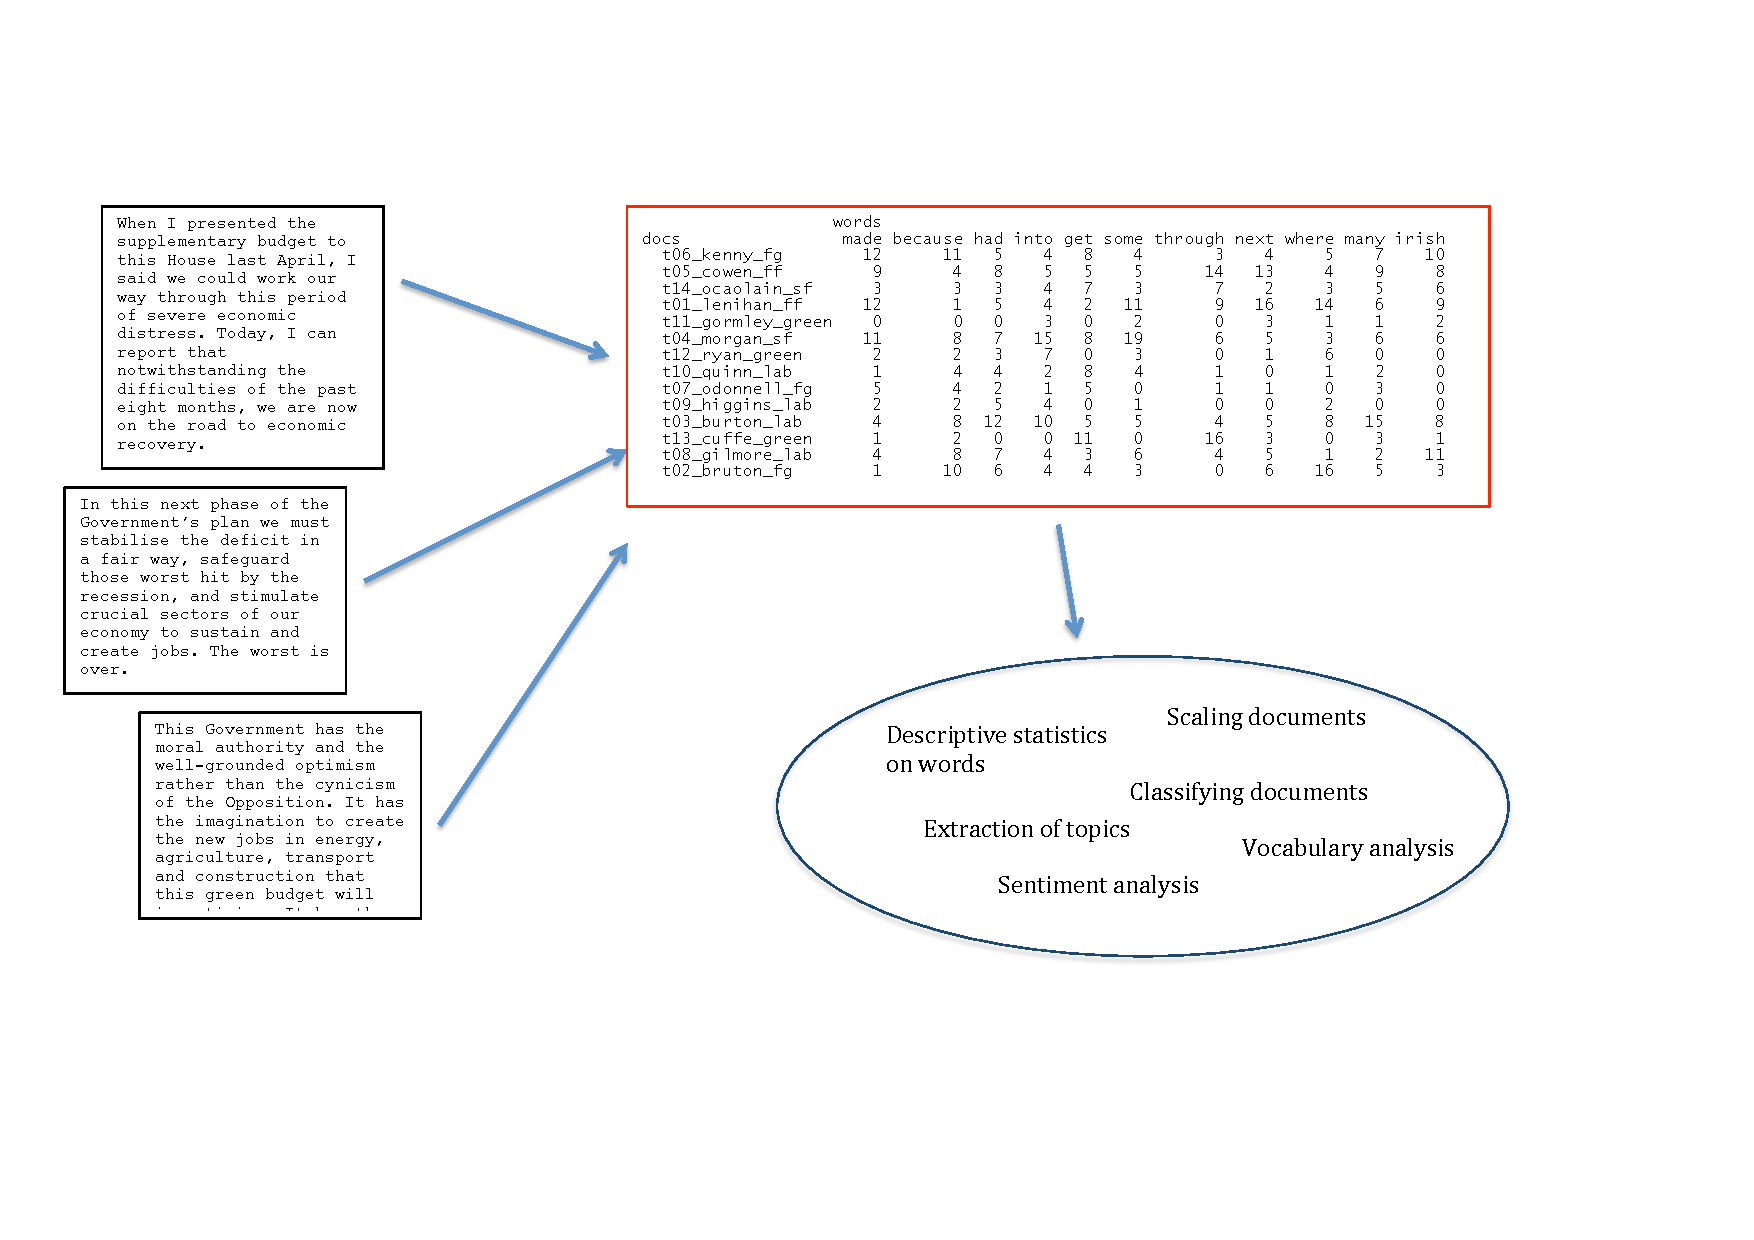
\includegraphics[width=11.5cm]{figures/workflow.pdf}
\end{frame}


\section{Fundamentals}

\begin{frame}[fragile]
	\frametitle{Some key basic concepts}
	\begin{description}[<+->]
		\item[(text) corpus] a large and structured set of texts for analysis
		\item[document] each of the units of the corpus
		\item[types] for our purposes, a unique word
		\item[tokens] any word -- so token count is total words
		\vspace{.20cm}
		\item[e.g.]
		\verb|A corpus is a set of documents.|
		\verb|This is the second document in the corpus.| \\
		\vspace{.20cm}
		\small{is a corpus with 2 documents, where each document is a sentence. The first document has 6 types and 7 tokens. The second has 7 types and 8 tokens. (We ignore punctuation for now.)}
		
	\end{description}
\end{frame}


\begin{frame}
	\frametitle{Some more key basic concepts}
	\begin{description}[<+->]
		\item[stems] words with suffixes removed (using set of rules)
		\item[lemmas] canonical word form (the base form of a word that has the same meaning even
		when different suffixes or prefixes are attached)\\
		\vspace{.20cm}
		\begin{tabular}{cccccc}
			\hline
			\textbf{word} &  win & winning & wins & won & winner \\
			\textbf{stem} & win & win & win & won & winner \\
			\textbf{lemma} & win & win & win & win & win \\
			\hline
		\end{tabular}
		\vspace{.20cm}
		\item[keys] such as dictionary entries, where the user
		defines a set of equivalence classes that group different word types
		\item[``key'' words] Words selected because of special
		attributes, meanings, or rates of occurrence
		\item[stop words] Words that are designated for exclusion
		from any analysis of a text    
	\end{description}
\end{frame}


% \begin{frame}
%   \centerline{\Large DEFINING ``DOCUMENTS''}
% \end{frame}


\begin{frame}
	\frametitle{Basic QTA adopts a bag-of-words approach}
	%  \vspace{-.5in}
	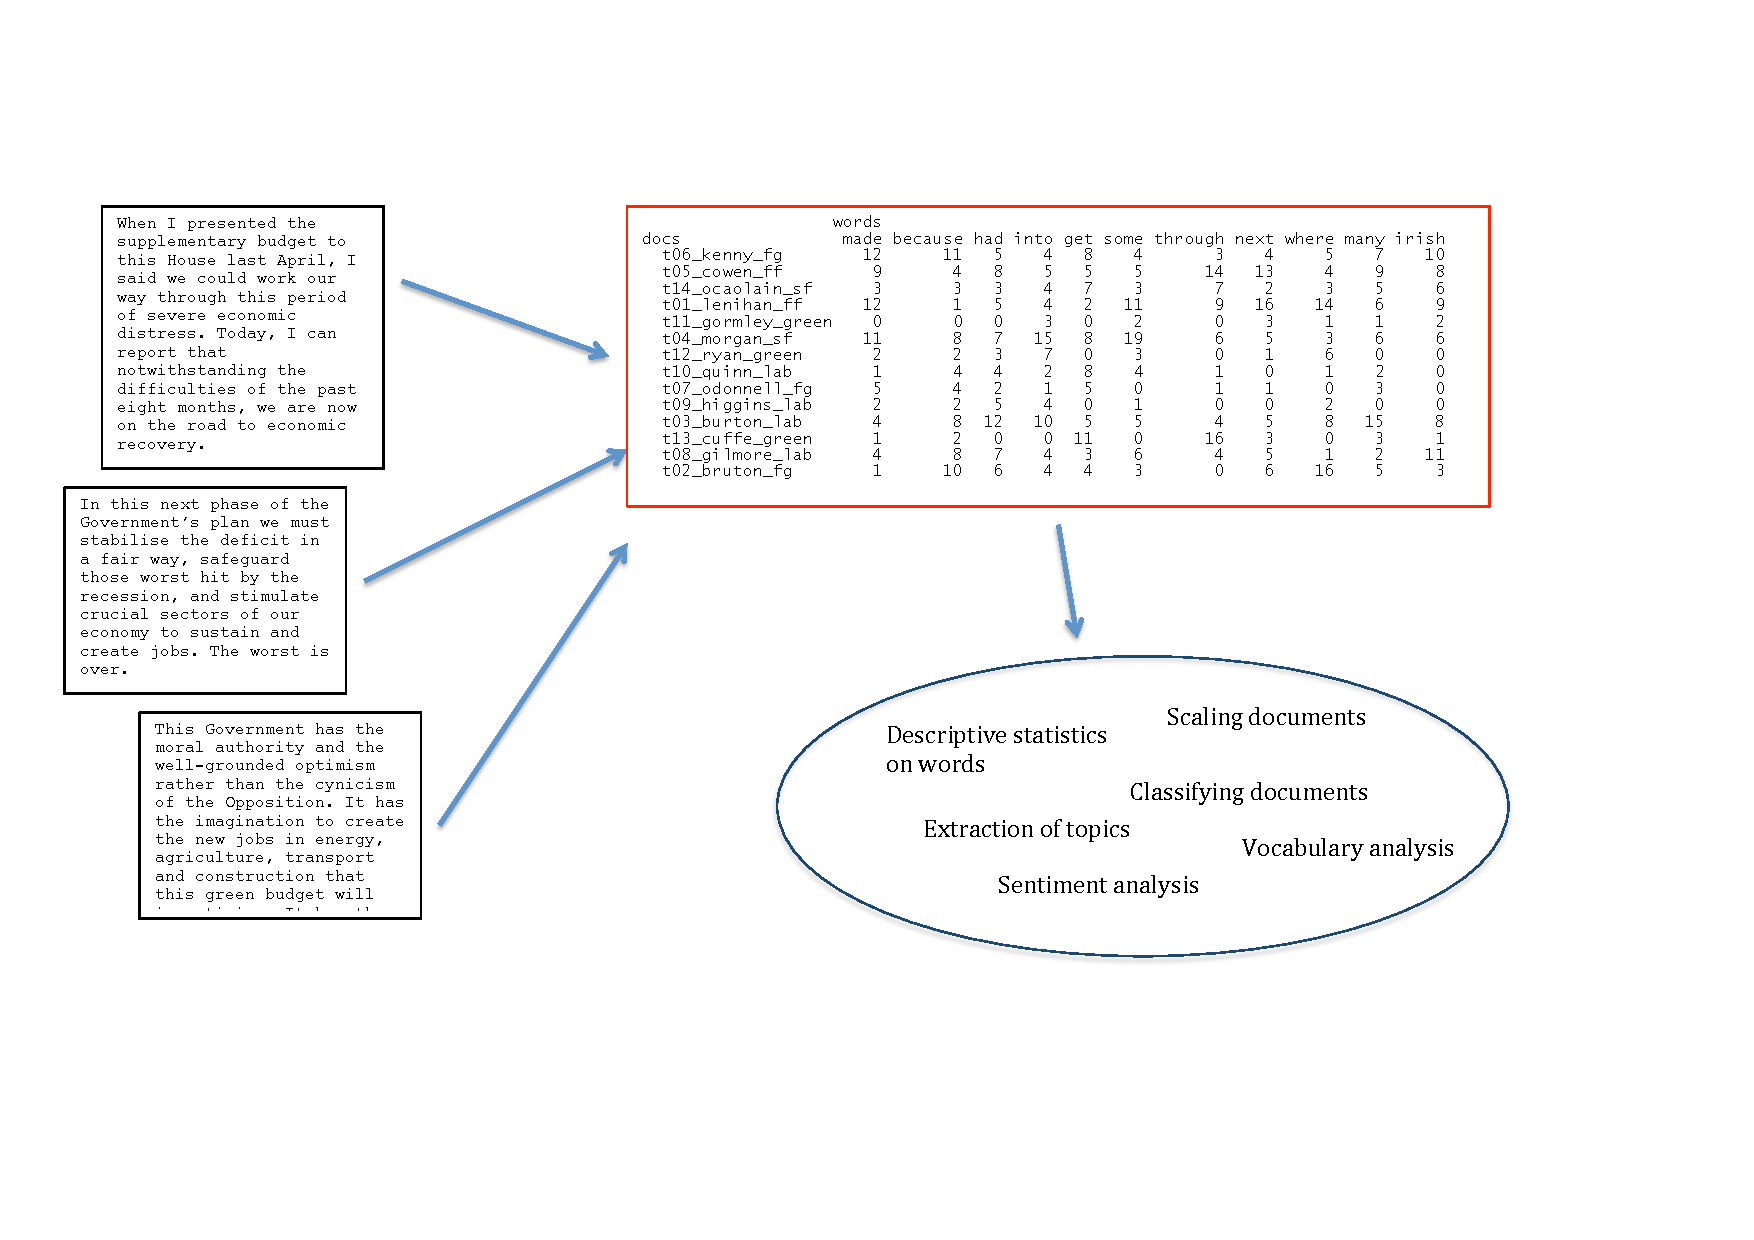
\includegraphics[width=11.5cm]{figures/workflow.pdf}
\end{frame}

\begin{frame}
	\frametitle{Bag-of-words approach}
	
	From words to numbers:
	\begin{enumerate}
		\item \alert{Preprocess text:} \uncover<2->{lowercase,} \uncover<3->{remove stopwords and punctuation,} \uncover<4->{stem,} \uncover<5->{tokenize into unigrams and bigrams (bag-of-words assumption)} \\
		\vspace{.10cm}
		\begin{footnotesize}
			\only<1>{``A corpus is a set of documents.''\\
				``This is the second document in the corpus.''}
			\only<2>{``\alert{a} corpus is a set of documents.''\\
				``\alert{t}his is the second document in the corpus.''}
			\only<3>{``\st{a} corpus \st{is} \st{a} set \st{of} documents\st{.}''\\
				``\st{this} \st{is} \st{the} second document \st{in} \st{the} corpus\st{.}''}
			\only<4>{``corpus set document\st{s}''\\
				``second document corpus''}
			\only<5->{[corpus, set, document, corpus set, set document] \newline
				[second, document, corpus, second document, document corpus]}
		\end{footnotesize}
		\item<6->\alert{Document-feature matrix}:
		\begin{itemize}
			\item $\mathbf{W}$: matrix of $N$ documents by $M$ unique n-grams
			\item $w_{im}$= number of times $m$-th n-gram appears in $i$-th document.\\
			\setlength{\tabcolsep}{3pt}
			\begin{footnotesize}
				\begin{tabular}{rcccccc}
					& \rotatebox[origin=l]{90}{corpus} & \rotatebox[origin=l]{90}{set} & \rotatebox[origin=l]{90}{document} & 
					\rotatebox[origin=l]	{90}{corpus set} &
					\rotatebox[origin=l]{90}{ \ldots} & \rotatebox[origin=l]{90}{$M$ n-grams} \\
					Document 1 & 1 & 1 & 1 & 1 &  \ldots \\
					\uncover<5->{Document 2 & 1 & 0 & 1 & 0 &  \ldots \\}
					\uncover<5->{\ldots \\}
					\uncover<5->{Document $n$ & 0 & 1 & 1 & 0 &  \ldots \\}
				\end{tabular}
				\setlength{\tabcolsep}{6pt}
			\end{footnotesize}
			
		\end{itemize}
	\end{enumerate}
\end{frame}

\begin{frame}
	\frametitle{Bag-of-words approach}
	\centering
	{\Large{QTA often disregards grammar and word order and uses word frequencies as features.\\ \vspace{.50cm} \alert{Why? What are the main advantages and limitations of this assumption?} }}
	
	
\end{frame}



\begin{frame}
	\frametitle{Word frequencies and their properties}
	Bag-of-words approach disregards grammar and word order and uses word frequencies as features. \alert{Why?} 
	\uncover<+->{
		\begin{itemize}[<+->]
			\item  \textit{Context is often uninformative}, conditional on presence of words:
			\begin{itemize}
				\item Individual word usage tends to be associated with a particular
				degree of affect, position, etc. without regard to context of word usage
			\end{itemize}
			\item  Single words tend to be the most informative, as 
			co-occurrences of multiple words ($n$-grams) are rare
			\item  Some approaches focus on occurrence of a word as a binary
			variable, irrespective of frequency: a binary outcome
			\item  Other approaches use frequencies: Poisson, multinomial, and
			related distributions 
	\end{itemize} }
\end{frame}



\begin{frame}
	\frametitle{Defining Features}
	\begin{itemize}[<+->]
		\item characters
		\item words
		\item  word stems or lemmas: this is a form of defining \emph{equivalence classes} for word features
		\item  word segments, especially for languages using compound words,
		such as German, e.g. \newline 
		\pause
		\htmladdnormallink{\emph{Rindfleischetikettierungsüberwachungsaufgabenübertragungsgesetz}}{http://www.telegraph.co.uk/news/worldnews/europe/germany/10095976/Germany-drops-its-longest-word-Rindfleischeti....html}
		\newline
		\pause {\footnotesize (the law concerning the delegation of duties for the supervision of cattle marking and the labelling of beef)} \newline
		\pause \emph{Saunauntensitzer}
	\end{itemize}
\end{frame}






\begin{frame}
	\frametitle{Strategies for feature selection}
	How to choose which features to include?
	\begin{itemize} [<+->]
		\item \alert{All?} Computationally inefficient, and rare words are generally uninformative
	\end{itemize}
	\uncover<+->{Potential criteria to select features (``trim'' the DFM):}
	\begin{itemize}[<+->]
		\item \alert{document frequency}: How many documents in which a term appears
		\item \alert{term frequency} How many times does the term appear in
		the corpus
		\item \alert{deliberate disregard}  Use of ``stop words'' -- words
		excluded because they represent linguistic connectors of no
		substantive content
		\item \alert{purposive selection} Use of a \emph{dictionary} of words or phrases
		\item \alert{declared equivalency classes} Non-exclusive synonyms,
		also known as \emph{thesaurus} (more on this later)
	\end{itemize}
\end{frame}

\begin{frame}[fragile]
	\frametitle{Common English stop words}
	\begin{small}
		\begin{verbatim}
		a, able, about, across, after, all, almost, also, am, among, 
		an, and, any, are, as, at, be, because, been, but, by, can, 
		cannot, could, dear, did, do, does, either, else, ever, 
		every, for, from, get, got, had, has, have, he, her, hers, 
		him, his, how, however, I, if, in, into, is, it, its, just, 
		least, let, like, likely, may, me, might, most, must, my, 
		neither, no, nor, not, of, off, often, on, only, or, other, 
		our, own, rather, said, say, says, she, should, since, so, 
		some, than, that, the, their, them, then, there, these, 
		they, this, tis, to, too, twas, us, wants, was, we, were, 
		what, when, where, which, while, who, whom, why, will, with, 
		would, yet, you, your 
		\end{verbatim}
	\end{small}
	\begin{itemize}
		\pause \item But no list should be considered universal
	\end{itemize}
\end{frame}


\begin{frame}
	\frametitle{A more comprehensive list of stop words}
	\begin{spacing}{.8}
		\tiny
		as, able, about, above, according, accordingly, across, actually, after, afterwards, again, against, ain't, all, allow, allows, almost, alone, along, already, also, although, always, am, among, amongst, an, and, another, any, anybody, anyhow, anyone, anything, anyway, anyways, anywhere, apart, appear, appreciate, appropriate, are, aren't, around, as, aside, ask, asking, associated, at, available, away, awfully, be, became, because, become, becomes, becoming, been, before, beforehand, behind, being, believe, below, beside, besides, best, better, between, beyond, both, brief, but, by, c'mon, c's, came, can, can't, cannot, cant, cause, causes, certain, certainly, changes, clearly, co, com, come, comes, concerning, consequently, consider, considering, contain, containing, contains, corresponding, could, couldn't, course, currently, definitely, described, despite, did, didn't, different, do, does, doesn't, doing, don't, done, down, downwards, during, each, edu, eg, eight, either, else, elsewhere, enough, entirely, especially, et, etc, even, ever, every, everybody, everyone, everything, everywhere, ex, exactly, example, except, far, few, fifth, first, five, followed, following, follows, for, former, formerly, forth, four, from, further, furthermore, get, gets, getting, given, gives, go, goes, going, gone, got, gotten, greetings, had, hadn't, happens, hardly, has, hasn't, have, haven't, having, he, he's, hello, help, hence, her, here, here's, hereafter, hereby, herein, hereupon, hers, herself, hi, him, himself, his, hither, hopefully, how, howbeit, however, i'd, i'll, i'm, i've, ie, if, ignored, immediate, in, inasmuch, inc, indeed, indicate, indicated, indicates, inner, insofar, instead, into, inward, is, isn't, it, it'd, it'll, it's, its, itself, just, keep, keeps, kept, know, knows, known, last, lately, later, latter, latterly, least, less, lest, let, let's, like, liked, likely, little, look, looking, looks, ltd, mainly, many, may, maybe, me, mean, meanwhile, merely, might, more, moreover, most, mostly, much, must, my, myself, name, namely, nd, near, nearly, necessary, need, needs, neither, never, nevertheless, new, next, nine, no, nobody, non, none, noone, nor, normally, not, nothing, novel, now, nowhere, obviously, of, off, often, oh, ok, okay, old, on, once, one, ones, only, onto, or, other, others, otherwise, ought, our, ours, ourselves, out, outside, over, overall, own, particular, particularly, per, perhaps, placed, please, plus, possible, presumably, probably, provides, que, quite, qv, rather, rd, re, really, reasonably, regarding, regardless, regards, relatively, respectively, right, said, same, saw, say, saying, says, second, secondly, see, seeing, seem, seemed, seeming, seems, seen, self, selves, sensible, sent, serious, seriously, seven, several, shall, she, should, shouldn't, since, six, so, some, somebody, somehow, someone, something, sometime, sometimes, somewhat, somewhere, soon, sorry, specified, specify, specifying, still, sub, such, sup, sure, t's, take, taken, tell, tends, th, than, thank, thanks, thanx, that, that's, thats, the, their, theirs, them, themselves, then, thence, there, there's, thereafter, thereby, therefore, therein, theres, thereupon, these, they, they'd, they'll, they're, they've, think, third, this, thorough, thoroughly, those, though, three, through, throughout, thru, thus, to, together, too, took, toward, towards, tried, tries, truly, try, trying, twice, two, un, under, unfortunately, unless, unlikely, until, unto, up, upon, us, use, used, useful, uses, using, usually, value, various, very, via, viz, vs, want, wants, was, wasn't, way, we, we'd, we'll, we're, we've, welcome, well, went, were, weren't, what, what's, whatever, when, whence, whenever, where, where's, whereafter, whereas, whereby, wherein, whereupon, wherever, whether, which, while, whither, who, who's, whoever, whole, whom, whose, why, will, willing, wish, with, within, without, won't, wonder, would, would, wouldn't, yes, yet, you, you'd, you'll, you're, you've, your, yours, yourself, yourselves, zero
	\end{spacing}
\end{frame}

\begin{frame}
	\frametitle{Stopwords}
	\centering
	{\Large{Are there cases in which we would want to keep stopwords? Or should we always exclude them from our analysis?}}
\end{frame}


\begin{frame}
	\frametitle{Stopwords sometimes can be informative!}
	
	\centering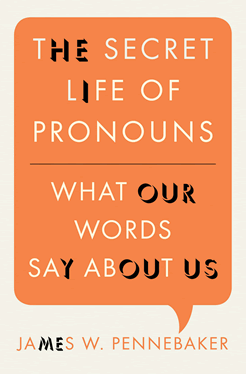
\includegraphics[height=.7\textheight]{figures/pennebaker.png} \\
	But sometimes we want to add/remove our own new stopwords (e.g. female pronouns, legislative terms, directional terms)
\end{frame}

\begin{frame}
	\frametitle{Stemming words}
	\begin{description}[<+->]
		\item[Lemmatization] refers to the algorithmic process of
		converting words to their lemma forms.  \pause 
		\item[stemming] the
		process for reducing inflected (or sometimes derived) words to
		their stem, base or root form.  Different from
		\emph{lemmatization} in that stemmers operate on single words
		without knowledge of the context.
		\item[both] convert the morphological variants into stem or root terms
		\item[example:]
		\alert{\texttt{produc}} from \newline
		\texttt{production, producer, produce, produces, produced}
		\item[Why?] Reduce feature space by collapsing different words into a stem (e.g. ``happier'' and ``happily'' convey same meaning as ``happy'')
	\end{description}
\end{frame}



\begin{frame}
	\frametitle{Wrapping up...}
	Big questions we answered today:
	
	\begin{itemize}
		\item Quantitative Text Analysis: why?
		\item Key terms: document, corpus, feature, document feature matrix, type, token

		\item How to select features? Bag-of-words, stemming, stopwords, part-of-speech tagging
	\end{itemize}

\end{frame}








\end{document} 